\textbf{COLUNI 2021 -- Questão 36}\par\medskip Ao longo das últimas décadas, as condições de vida no Brasil se transformaram. A medicina teve avanços importantes, novas vacinas, fármacos e tratamentos médicos foram desenvolvidos e possibilitaram a melhoria das condições de vida da população mundial. Também houve redução no número de pessoas que passam fome no mundo, e, no Brasil, a luta contra a fome gerou resultados positivos. A partir dessas informações, leia atentamente os gráficos abaixo:

\par

\textbf{GRÁFICO I}

% COLUNI-AUTO-FIGURES-BEGIN
\begin{figure}[htbp]
\centering
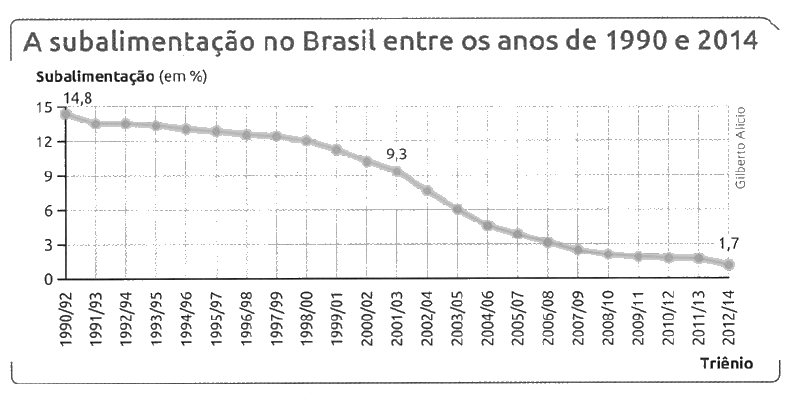
\includegraphics[width=0.95\linewidth]{static/simulados/coluni/figuras/2021/questao-36/figura-1.png}
\end{figure}
% COLUNI-AUTO-FIGURES-END

CHIBA, Charles; MINORELLI, Caroline. \textbf{Convergências}: história, 9° ano: anos finais do ensino fundamental. São Paulo: Edições SM, 2016, p. 234.

\par

\textbf{GRÁFICO II}

% COLUNI-AUTO-FIGURES-BEGIN
\begin{figure}[htbp]
\centering
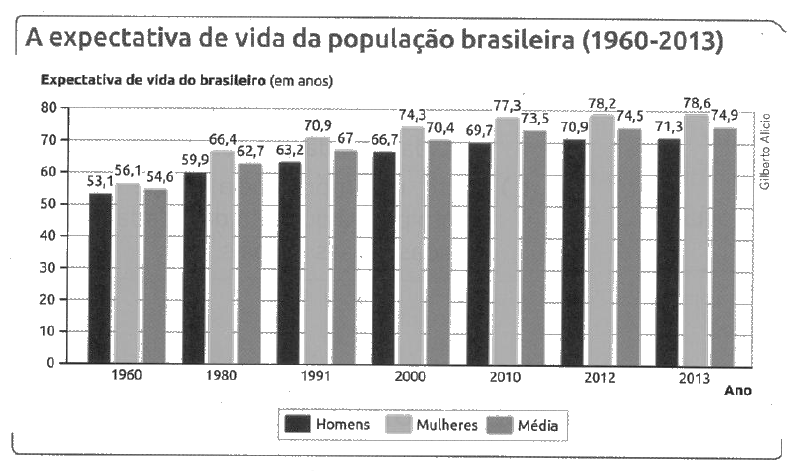
\includegraphics[width=0.95\linewidth]{static/simulados/coluni/figuras/2021/questao-36/figura-2.png}
\end{figure}
% COLUNI-AUTO-FIGURES-END

CHIBA, Charles; MINORELLI, Caroline. \textbf{Convergências}: história, 9° ano: anos finais do ensino fundamental. São Paulo: Edições SM, 2016, p. 235.

\par

Sobre as mudanças ocorridas no Brasil entre os séculos XX e XXI, é INCORRETO afirmar que:


\begin{enumerate}
\item A primeira década do século XXI foi marcada por vertiginosa queda nos dados da subalimentação no
      Brasil, indicando resultados positivos da luta contra a fome no país.
\item O uso de antibióticos e vacinas, a adoção de medidas preventivas no sistema de saúde pública e a
      expansão da rede de saneamento básico foram essenciais na melhoria das condições de vida no Brasil.
\item A expectativa de vida e, por consequência, o número de idosos no Brasil aumentaram entre os séculos
      XX e XXI, demandando menos atenção do Poder Público a essa parcela da população.
\item O Brasil avançou no combate à fome, mas ainda é preciso melhorar a qualidade da alimentação e reduzir
      o consumo de gordura, açúcar e sal que, em excesso, podem provocar doenças como diabetes e
      obesidade.\end{enumerate}
